\documentclass[12pt, twoside]{article}
\usepackage[letterpaper, margin=1in, headsep=0.5in]{geometry}
\usepackage[english]{babel}
\usepackage[utf8]{inputenc}
\usepackage{amsmath}
\usepackage{amsfonts}
\usepackage{amssymb}
\usepackage{tikz}
\usetikzlibrary{quotes, angles}
\usepackage{graphicx}
\usepackage{enumitem}
\usepackage{multicol}

\newif\ifmeta
\metatrue %print standards and topics tags

\title{Regents Geometry}
\author{Chris Huson}
\date{January 2022}

\usepackage{fancyhdr}
\pagestyle{fancy}
\fancyhf{}
\renewcommand{\headrulewidth}{0pt} % disable the underline of the header
\raggedbottom

\fancyhead[LE]{\thepage}
\fancyhead[RO]{\thepage \\ Name: \hspace{4cm} \,\\}
\fancyhead[LO]{BECA / Dr. Huson / Geometry 6 Trigonometry}

\begin{document}
\subsubsection*{6.9 Classwork: Unit circle \hfill CCSS.HSG.SRT.C.8}
\begin{enumerate}
  \item Do Now: A vector from the origin $\overrightarrow{OA}$ is shown rotated counterclockwise around $O$.
  \begin{multicols}{2}
        \begin{enumerate}
        \item Using a protractor, measure the angle of rotation.
        \item Write down the slope of $\overrightarrow{OA'}$.
        \item Mark and label the point $B(4,-3)$. Draw $\overrightarrow{OB}$.
        \item Write down the slope of $\overrightarrow{OB}$.
        \item What is the product of the slopes of $\overrightarrow{OA'}$ and $\overrightarrow{OB}$?
      \end{enumerate}
      \begin{center}
      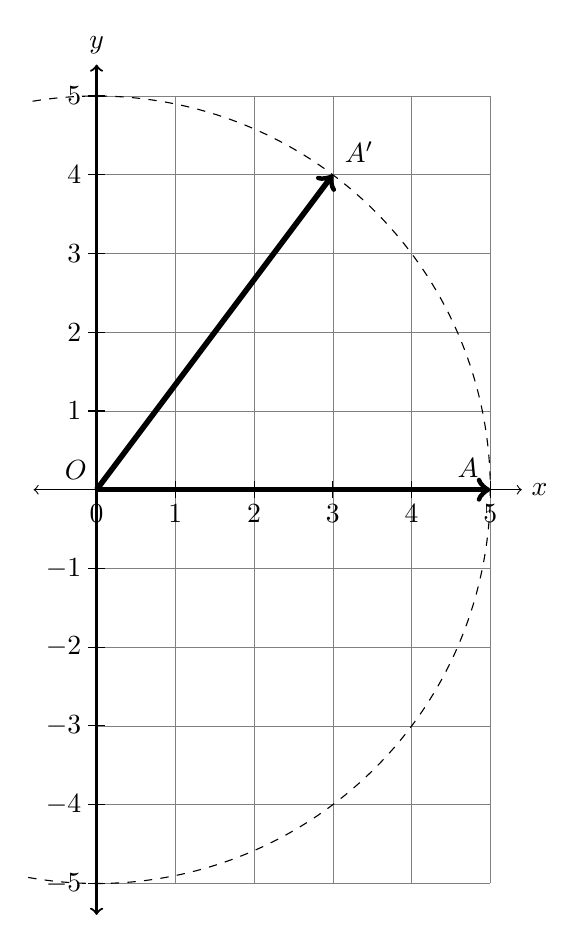
\begin{tikzpicture}[scale=1]
      \draw [help lines] (0,-5) grid (5,5);
      \draw [<->] (-0.8,0) -- (5.4,0) node [right] {$x$};
      \draw [thick, <->] (0,-5.4)--(0,5.4) node [above] {$y$};
      \foreach \x in {0,1,2,3,4,5}
        \draw[shift={(\x,0)},color=black] (0pt,-3pt) -- (0pt,3pt) node[below=5pt]  {$\x$};
      \foreach \y in {-5,...,-1,1,2,3,4,5}
        \draw[shift={(0,\y)},color=black] (-3pt,0pt) -- (3pt,0pt) node[left=5pt]  {$\y$};
      %\draw [dashed] (0,0) circle [radius=5cm];
      \draw [dashed] (-100:5) arc (-100:100:5);
      \node at (0,0)[above left]{$O$};
      \draw [line width=2pt, ->] (0,0)--(5,0) node [above left] {$A$};
      \draw [line width=2pt, ->] (0,0)--(3,4) node [above right] {$A'$};
    \end{tikzpicture}
  \end{center}
\end{multicols}

\item Complete the table mapping angle of rotation onto slope. (six entries)\\
      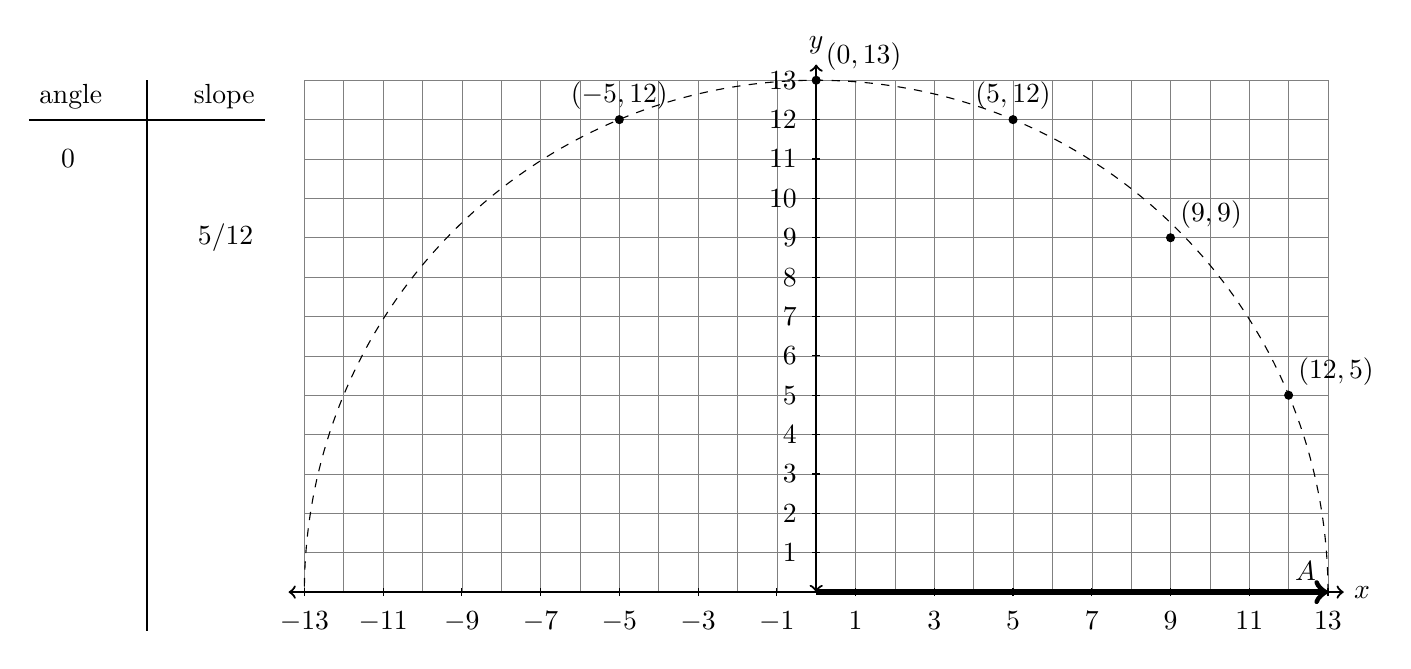
\begin{tikzpicture}[scale=0.5]
      \draw [help lines] (-13,0) grid (13,13);
      \draw [thick, <->] (-13.4,0) -- (13.4,0) node [right] {$x$};
      \draw [thick, <->] (0,0)--(0,13.4) node [above] {$y$};
      \foreach \x in {-13,-11,...,13}
        \draw[shift={(\x,0)},color=black] (0pt,-3pt) -- (0pt,3pt) node[below=5pt]  {$\x$};
      \foreach \y in {1,...,13}
        \draw[shift={(0,\y)},color=black] (-3pt,0pt) -- (3pt,0pt) node[left=5pt]  {$\y$};
      %\draw [dashed] (0,0) circle [radius=5cm];
      \draw [dashed] (0:13) arc (0:180:13);
      \draw [line width=2pt, ->] (0,0)--(13,0) node [above left] {$A$};
      \draw [fill] (12,5) circle [radius=0.1cm] node[above right]{$(12,5)$};
      \draw [fill] (5,12) circle [radius=0.1cm] node[above]{$(5,12)$};
      \draw [fill] (-5,12) circle [radius=0.1cm] node[above]{$(-5,12)$};
      \draw [fill] (9,9) circle [radius=0.1cm] node[above right]{$(9,9)$};
      \draw [fill] (0,13) circle [radius=0.1cm] node[above right]{$(0,13)$};

      \draw [thick] (-20,12) node [above right] {angle} -- (-14,12) node [above left] {slope};
      \draw [thick] (-17,13)--(-17,-1);
      \node at (-19,11){$0$};
      \node at (-15,9){$5/12$};
    \end{tikzpicture}

  \newpage
  \subsubsection*{Mastery topic: Algebraic solution \hfill (2 stars each)}
  \item Solve each equation for $x$, rounding to the nearest hundredth.
    \begin{enumerate}
    \begin{multicols}{2}
    \item $\displaystyle \tan 63^\circ = \frac{x}{14}$ \vspace{5cm}
    \item $\displaystyle \tan 77^\circ = \frac{10}{x}$
    \item $\displaystyle \sin 46^\circ  = \frac{x}{3.5}$ \vspace{5cm}
    \item $\displaystyle \cos 35^\circ = \frac{x}{21}$ 
    \end{multicols}
  \end{enumerate}
    \vspace{6cm}
  \item Solve for $x$, rounding to the nearest whole degree.
    \begin{enumerate}
    \begin{multicols}{2}
    \item $\displaystyle x = \tan^{-1} (\frac{12}{5})$ \vspace{4cm}
    \item $\displaystyle \tan x^\circ = \frac{3.2}{4.8}$ \vspace{4cm}
    \end{multicols}
  \end{enumerate}
  
  \newpage
  \subsubsection*{Mastery topic: Calculator use}
    \item Express the result to the nearest thousandth. \hfill (1 star each) \vspace{.5cm}
      \begin{multicols}{2}
        \begin{enumerate}
          \item $\tan 22^\circ = $ \vspace{1cm}
          \item $\tan 81^\circ =$
          \item $\tan 15^\circ = $ \vspace{1cm}
          \item $\tan 65^\circ =$
        \end{enumerate}
      \end{multicols} \vspace{1cm}
  
    \item Round each value to the nearest degree. \hfill (1 star each) \vspace{.5cm}
    \begin{multicols}{2}
      \begin{enumerate}
        \item $\tan^{-1} (2) = $ \vspace{1cm}
        \item $\tan^{-1} (0.5) =$
        \item $\tan^{-1} (1) = $ \vspace{1cm}
        \item $\tan^{-1} (\sqrt{3}) =$
      \end{enumerate}
    \end{multicols} \vspace{1cm}
  
    \item Round each value to the nearest hundredth. \hfill (2 stars each) \vspace{.5cm}
    \begin{multicols}{2}
      \begin{enumerate}
        \item $AB=\sqrt{11^2+7^2}$ \vspace{3.5cm}
        \item $AB=\sqrt{3.2^2+1.9^2}$
        \item $AB=\sqrt{(-8.0)^2+(14.5)^2}$ \vspace{3.5cm}
        \item $AB=\sqrt{(4-3)^2+(7-11)^2}$
      \end{enumerate}
    \end{multicols} \vspace{1cm}
  
  \newpage  
  \subsubsection*{Modeling: Mark each diagram and write and equation. Do Not Solve!}
  Write an equation expressing $\tan (\angle)$ as a ratio of \emph{opposite} over \emph{adjacent}. 
    \item Given right $\triangle JKL$ with $\overline{JK} \perp \overline{KL}$, $JK=8$, $m\angle J=24^\circ$. Let $x$ be the length of the side opposite $\angle J$, $x=KL$.  \hfill (2 stars)
        \begin{flushright}
            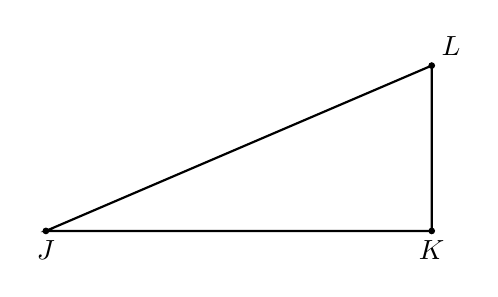
\begin{tikzpicture}[scale=0.7]
              \draw [thick](-1,0)--(6,0)--(6,3)--cycle;
              \draw [fill] (-1,0) circle [radius=0.05] node[below]{$J$};
              \draw [fill] (6,0) circle [radius=0.05] node[below]{$K$};
              \draw [fill] (6,3) circle [radius=0.05] node[above right]{$L$};
            \end{tikzpicture}
          \end{flushright}
  
    \item Given right $\triangle ABC$ with $m\angle C =90^\circ$, $BC=15$, $m\angle A=41^\circ$. Let $x=AC$. \hfill (2 stars)
      \begin{flushright}
          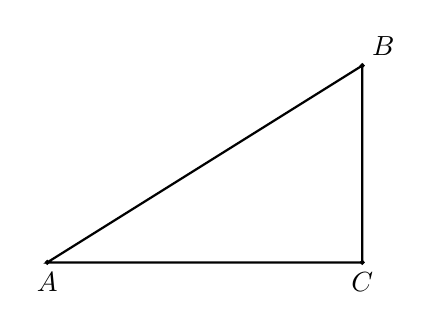
\begin{tikzpicture}[scale=0.5]
            \draw [thick](-1,0)--(7,0)--(7,5)--cycle;
            \draw [fill] (-1,0) circle [radius=0.05] node[below]{$A$};
            \draw [fill] (7,0) circle [radius=0.05] node[below]{$C$};
            \draw [fill] (7,5) circle [radius=0.05] node[above right]{$B$};
          \end{tikzpicture}
        \end{flushright}
  
    \item Given right $\triangle ABC$ with $m\angle C =90^\circ$, $BC=4$, $AC=19$, and $m\angle A=x^\circ$. \hfill (2 stars)
    \begin{flushright}
      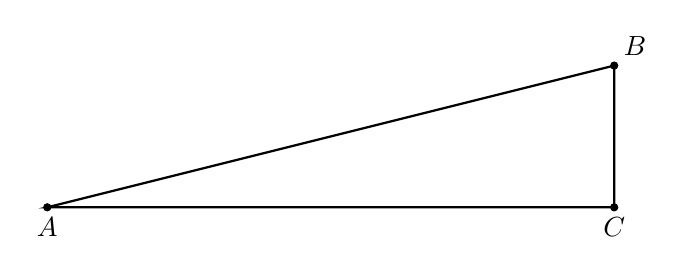
\begin{tikzpicture}[scale=0.9]
        \draw [thick](-1,0)--(7,0)--(7,2)--cycle;
        \draw [fill] (-1,0) circle [radius=0.05] node[below]{$A$};
        \draw [fill] (7,0) circle [radius=0.05] node[below]{$C$};
        \draw [fill] (7,2) circle [radius=0.05] node[above right]{$B$};
      \end{tikzpicture}
    \end{flushright}
    
    \item Given right $\triangle ABC$ with $\overline{AC} \perp \overline{BC}$, $BC=7$, $m\angle B=55^\circ$. Let $x=AC$. \hfill (3 stars)
    \begin{flushright}
      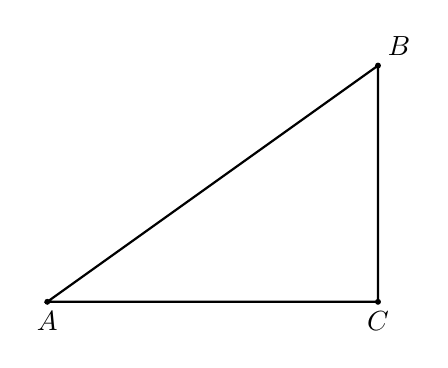
\begin{tikzpicture}[scale=0.6]
        \draw [thick](-1,0)--(6,0)--(6,5)--cycle;
        \draw [fill] (-1,0) circle [radius=0.05] node[below]{$A$};
        \draw [fill] (6,0) circle [radius=0.05] node[below]{$C$};
        \draw [fill] (6,5) circle [radius=0.05] node[above right]{$B$};
      \end{tikzpicture}
    \end{flushright}
  
\end{enumerate}
\end{document}
